\documentclass[11pt,a4paper]{article}

% ---------- Layout and typography ----------
\usepackage[T1]{fontenc}
\usepackage[utf8]{inputenc}
\usepackage[margin=25mm]{geometry}
\usepackage{newtxtext,newtxmath}
\usepackage{microtype}
\usepackage{graphicx}
\usepackage{booktabs}
\usepackage{tabularx}
\usepackage{multirow}
\usepackage{array}
\usepackage{xcolor}
\usepackage{enumitem}
\usepackage[font=small,labelfont=bf,skip=6pt]{caption}
\usepackage{subcaption}
\usepackage[numbers,sort&compress]{natbib}
\usepackage[colorlinks=true,linkcolor=accent,citecolor=accent,urlcolor=accent]{hyperref}

\definecolor{accent}{HTML}{1F4E79}
\graphicspath{{figures/}}
\setlength{\parskip}{2pt plus 1pt}
\emergencystretch=1.5em
\makeatletter\setlength{\@fptop}{0pt}\makeatother
\renewcommand{\arraystretch}{1.15}
\newcolumntype{Y}{>{\centering\arraybackslash}X}
\newcolumntype{L}{>{\raggedright\arraybackslash}X}
\newcommand{\best}[1]{\textbf{#1}}
\newcommand{\second}[1]{\underline{#1}}
\setlist{nosep,leftmargin=1.4em}
% One appendix example: the description and its figure form a single block that
% is never split across pages. Arguments: title, label, image, caption, text.
\newcommand{\qualexample}[5]{%
  \par\noindent
  \begin{minipage}{\linewidth}
    \paragraph{#1 (Figure~\ref{#2}).} #5\par
    \vspace{7pt}
    \centering
    \includegraphics[width=\qualwidth]{#3}
    \captionof{figure}{#4}\label{#2}
  \end{minipage}%
  \par\vspace{14pt plus 6pt minus 3pt}}
\newcommand{\qualwidth}{0.86\linewidth}

% ---------- Fill in before submission ----------
\newcommand{\groupid}{Group 11}
\newcommand{\memberA}{Liu Shiyuan}  \newcommand{\matricA}{Matric No.\ G2509682L}
\newcommand{\memberB}{Luo Zhiyuan}  \newcommand{\matricB}{Matric No.\ G2509624F}
\newcommand{\memberC}{Zhang Wei}  \newcommand{\matricC}{Matric No.\ G2610110E}
\newcommand{\memberD}{Zhang Mufan}  \newcommand{\matricD}{Matric No.\ G2505269G}

\begin{document}

% ---------- Title block ----------
\begin{center}
  {\small\scshape AI6132 \,\textperiodcentered\, Project 1 \,\textperiodcentered\, Technical Review \,\textperiodcentered\, \groupid}\\[10pt]
  {\LARGE\bfseries Review of Image-to-Video Generation:\\[4pt]
   A Controlled Comparison of Four Open-Source Models}\\[16pt]
  \begin{tabular}{@{}c@{\hspace{7mm}}c@{\hspace{7mm}}c@{\hspace{7mm}}c@{}}
    \textbf{\memberA} & \textbf{\memberB} & \textbf{\memberC} & \textbf{\memberD}\\
    \small\matricA & \small\matricB & \small\matricC & \small\matricD\\
  \end{tabular}\\[10pt]
  {\small College of Computing and Data Science, Nanyang Technological University}\\[2pt]
  {\small November 2026}
\end{center}
\vspace{4pt}

\begin{abstract}
\noindent
Open-source image-to-video (I2V) generators have improved quickly, but published results are rarely comparable because each model is reported with its own inputs, clip length and metrics. We compare four recent diffusion-transformer models, Wan~2.2, HunyuanVideo~1.5, LTX-Video and LongCat-Video, on the same 24 reference images and prompts from VBench-I2V with a fixed seed, producing 96 videos: 18 short clips of about 129 frames and 6 long clips of about 513 frames per model. Each video is scored by four human raters on four criteria, by the VBench-I2V automatic metrics, and by a Qwen3-VL judge. On short clips all four models score well (mean human scores of 3.3 to 4.9 out of 5). Long clips separate them: LTX-Video stays within 0.44 points of its short-clip scores on every criterion, whereas Wan~2.2 and LongCat-Video fall below 2.0 on image alignment and background preservation. LTX-Video is also the cheapest model to run, at 25\,s per short clip against 173 to 464\,s for the others. The automatic evaluators agree with human raters only in part. The Qwen3-VL judge tracks human scores on image alignment (Spearman $\rho=0.60$) and prompt adherence ($\rho=0.51$), but its motion scores are uncorrelated with human judgement ($\rho=-0.06$). The comparison covers one seed and a fixed set of 24 cases, and the models ran at different step counts and resolutions, so the results describe these configurations rather than the model families in general.
\end{abstract}

% =====================================================================
\section{Introduction}
Image-to-video generation takes a reference image, usually together with a text prompt, and produces a video that starts from that image. The task is harder to evaluate than text-to-video generation because the output has to satisfy three constraints at once: it must stay faithful to the given image, follow the prompt, and move plausibly over time. A model can satisfy one constraint by sacrificing another. A nearly static video preserves the reference image perfectly, and a video with vigorous motion often does so by letting the subject or the background drift.

Recent open-source systems share a common design, a latent diffusion transformer~\citep{peebles2023dit} trained with a flow-matching objective~\citep{lipman2023flow} on top of a spatio-temporal video autoencoder, yet they differ in model size, latent compression and sampling budget. Their papers report results under different settings, which makes it difficult to tell how they rank on the same inputs. This report therefore runs a small controlled comparison and asks three questions.
\begin{enumerate}
  \item How well does each model preserve the reference image, follow the prompt and produce natural motion on identical inputs?
  \item How do these properties change when the clip is extended from about 5 seconds to about 20 seconds?
  \item How far do automatic evaluators, namely VBench-I2V~\citep{huang2024vbench,huang2024vbenchpp} and a vision-language model (VLM) judge, agree with human raters?
\end{enumerate}

Our main findings are that the four models are close on short clips and far apart on long ones, that the fastest model in our setting is also the one that degrades least, and that neither automatic evaluator is a reliable substitute for human judgement of motion.

% =====================================================================
\section{Background and Models}
\label{sec:models}

\paragraph{I2V with diffusion transformers.}
Early open I2V systems such as Stable Video Diffusion~\citep{blattmann2023svd} extended image diffusion U-Nets with temporal layers. Current models instead denoise a compressed spatio-temporal latent with a transformer, as in HunyuanVideo~\citep{kong2024hunyuanvideo}. The reference image is typically encoded into the first latent frame, and the model generates the remaining frames conditioned on it and on text embeddings. Sampling cost is governed by the number of latent tokens and the number of denoising steps, and step distillation~\citep{salimans2022progressive} reduces the latter from about 50 steps to fewer than 20, usually while removing classifier-free guidance~\citep{ho2022cfg}. Three of the four checkpoints in this study are distilled.

\paragraph{Wan~2.2.}
Wan~\citep{wan2025} is a family of flow-matching video transformers. We use the Wan2.2-TI2V-5B checkpoint, a 5-billion-parameter model that handles text-to-video and image-to-video in one network. It relies on a high-compression autoencoder with a $4\times16\times16$ compression ratio and a umT5-XXL text encoder, and it targets 720p output at 24\,fps. It is the only non-distilled checkpoint in the comparison.

\paragraph{HunyuanVideo~1.5.}
HunyuanVideo~1.5~\citep{hunyuanvideo15} is an 8.3-billion-parameter successor to HunyuanVideo~\citep{kong2024hunyuanvideo} that uses a multimodal large language model as its text encoder and a vision encoder for image conditioning. We use the official 480p I2V step-distilled checkpoint, which samples in 8 steps.

\paragraph{LTX-Video.}
LTX-Video~\citep{hacohen2024ltx} is designed for speed. Its autoencoder compresses video far more aggressively than the others, and the final denoising step is moved into the decoder to recover fine detail. We use the 13B v0.9.8 distilled checkpoint with its official two-stage schedule, in which 7 steps at reduced resolution are followed by latent upsampling and 3 refinement steps.

\paragraph{LongCat-Video.}
LongCat-Video~\citep{longcat2025} is a 13.6-billion-parameter model that handles text-to-video, image-to-video and video continuation in a single network and is intended for minutes-long generation. We use the base checkpoint with the official CFG- and step-distillation LoRA, which samples in 16 steps.

% =====================================================================
\section{Experimental Setup}
\label{sec:setup}

\subsection{Test Set}
The test set consists of 24 image--prompt pairs taken from the 16:9 crops of VBench-I2V~\citep{huang2024vbenchpp} and selected manually to cover 11 content categories (Figure~\ref{fig:dataset}). Single-person and multiple-person scenes contribute three cases each and the other nine categories two each. Sixteen cases are subject-centred and eight are background-centred (architecture, scenery, indoor and abstract). Six cases, one from each of six categories, are designated long clips. The prompts are the original VBench captions and are used without rewriting or prompt extension.

\begin{figure}[!tb]
  \centering
  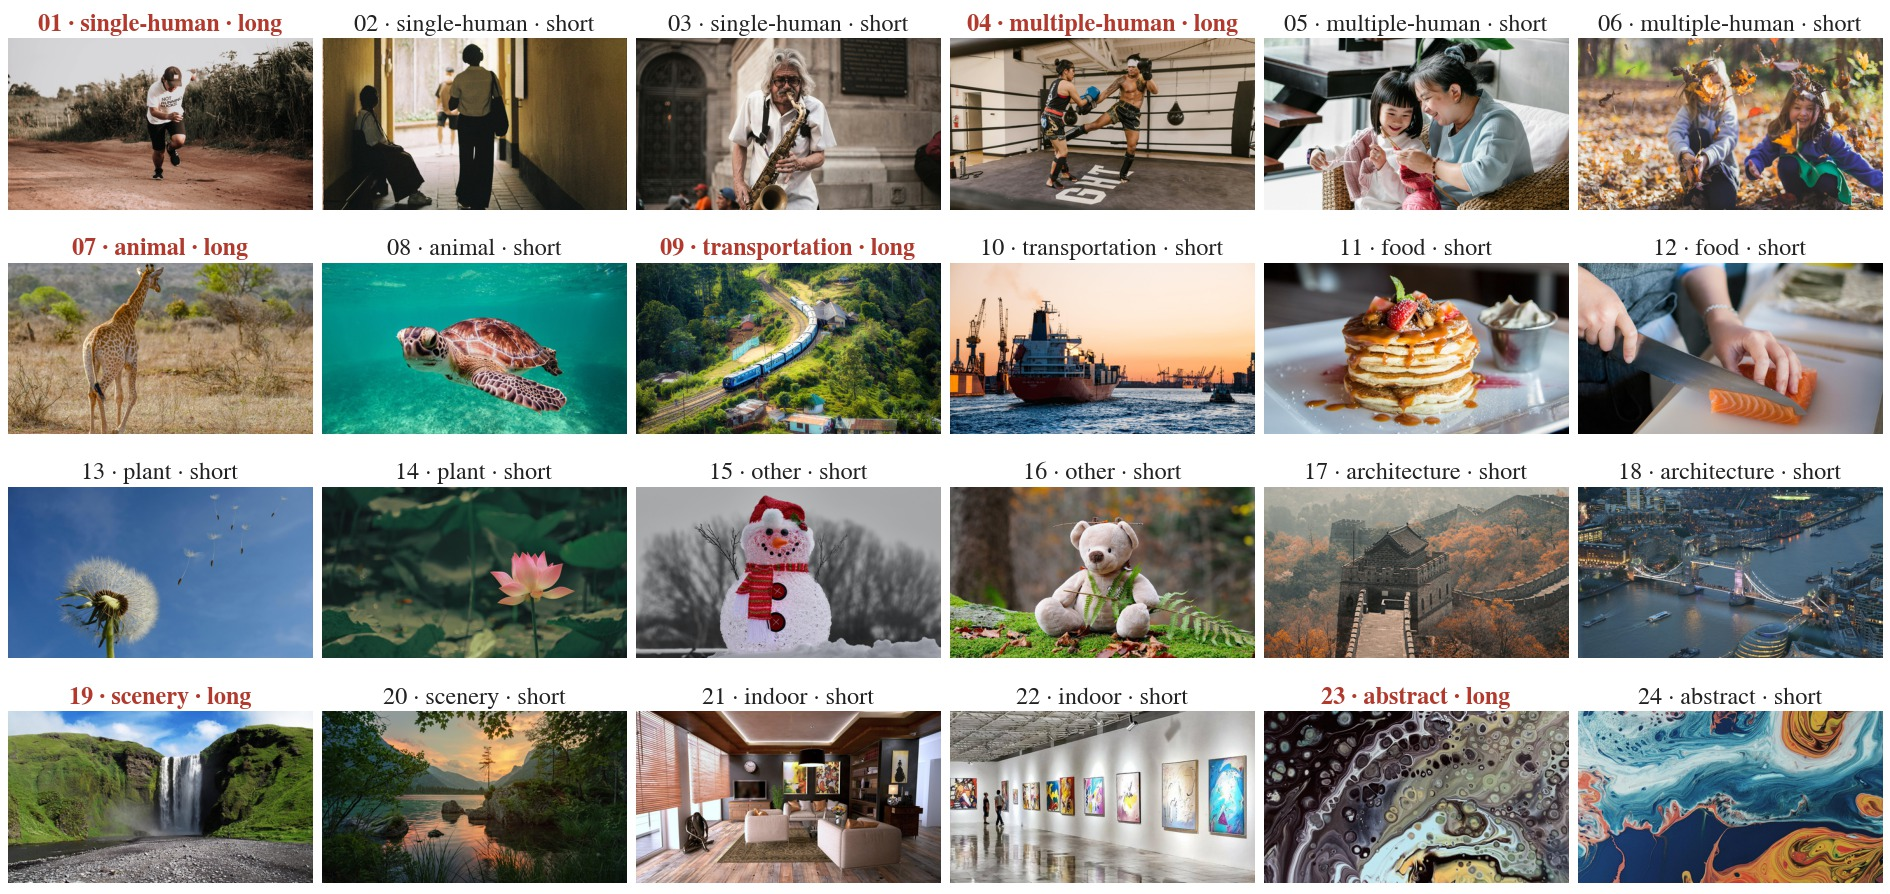
\includegraphics[width=\linewidth]{dataset_overview.jpg}
  \caption{The 24 reference images with their case number, VBench-I2V category and clip length. The six long cases (red) target 513 frames and the remaining 18 target 129 frames.}
  \label{fig:dataset}
\end{figure}

\subsection{Generation Protocol}
Every model receives the same image, prompt and seed (42) and generates each case once, giving $24\times4=96$ videos with no retries or selection. Short clips target 129 frames and long clips 513 frames, generated in a single pass. Each team member ran one model with the settings in Table~\ref{tab:config}. All 96 generations completed and decoded successfully.

The settings are not identical across models, and three deviations matter for interpretation. First, Wan~2.2 was run with 10 denoising steps instead of its default 50, and produced 125 and 509 frames instead of 129 and 513. Second, Wan~2.2 generates at $1248\times704$, about 2.2 times the pixel count of the 480p models. Third, LongCat-Video outputs 15\,fps, so its clips last 8.6\,s and 34.2\,s for the same number of frames. A 513-frame clip is also several times longer than the default clip length of every model, so the long-clip results should be read as a stress test of temporal extrapolation.

\begin{table}[!htb]
  \centering
  \small
  \caption{Checkpoints and inference settings. Frames and durations are given as short\,/\,long. All models use BF16 weights, seed 42 and no prompt extension.}
  \label{tab:config}
  \begin{tabularx}{\linewidth}{@{}l L c c c c c c@{}}
    \toprule
    Model & Checkpoint & Params & Steps & CFG & Resolution & FPS & Frames \\
    \midrule
    Wan~2.2          & Wan2.2-TI2V-5B                         & 5B    & 10    & 5.0 & $1248\times704$ & 24 & 125\,/\,509 \\
    HunyuanVideo~1.5 & 480p I2V, step-distilled               & 8.3B  & 8     & --  & $848\times480$  & 24 & 129\,/\,513 \\
    LTX-Video        & 13B v0.9.8, distilled                  & 13B   & 7+3   & 1.0 & $768\times432$  & 24 & 129\,/\,513 \\
    LongCat-Video    & Base + CFG-step distillation LoRA      & 13.6B & 16    & 1.0 & $832\times480$  & 15 & 129\,/\,513 \\
    \bottomrule
  \end{tabularx}
\end{table}

\subsection{Evaluation}
\label{sec:evaluation}

\paragraph{Human rating.}
All four team members rated all 96 videos, giving 384 rating records and 1{,}536 scores with no missing values. Videos were presented under anonymous identifiers in a different random order for each rater, next to the reference image and the prompt, in an offline web viewer. Each video receives four integer scores from 1 to 5:
\begin{description}[leftmargin=1.4em,itemsep=1pt]
  \item[Image alignment.] Whether the appearance of the subject and scene in the reference image stays stable. A score of 1 means the subject is replaced or unrecognisable.
  \item[Motion naturalness.] Whether motion is continuous and physically plausible. A score of 1 means severe stutter, structural deformation, or a requested action that is largely absent.
  \item[Prompt adherence.] Whether the subject, action and scene named in the prompt can be verified in the video.
  \item[Background preservation.] Whether background structure, edges and texture remain as detailed as in the reference image for the whole clip.
\end{description}
The full anchors are listed in Appendix~\ref{app:rubric}. For each video and criterion we take the median of the four raters, and we report the mean of these medians over a model's videos. Rater agreement is measured with ordinal Krippendorff's $\alpha$~\citep{krippendorff2011}. Because each rater generated one of the models and the staged delivery of videos reduced anonymity, the evaluation is not fully blind. We therefore also recompute every score without the rater who ran the model in question.

\paragraph{VBench-I2V.}
We run the official VBench-I2V implementation~\citep{huang2024vbenchpp} on full-length $768\times432$, 12\,fps copies of every video. \emph{I2V subject} and \emph{I2V background} combine the feature similarity between the reference image and the frames with the similarity between adjacent frames, using DINO~\citep{caron2021dino} and DreamSim~\citep{fu2023dreamsim} features respectively. \emph{Motion smoothness} measures how well a frame-interpolation model~\citep{li2023amt} predicts dropped frames, and \emph{dynamic degree} is the fraction of clips whose optical flow~\citep{teed2020raft} exceeds a threshold. Following the benchmark, subject, smoothness and dynamic degree are computed on the 16 subject cases and background on the 8 background cases, which gives 224 metric values in total.

\paragraph{VLM judge.}
VLM-based scoring is attractive as a scalable proxy for human rating~\citep{he2024videoscore}, so we test how far it can be trusted here. We use Qwen3-VL-32B-Instruct~\citep{qwen3vl} with 4-bit NF4 quantisation and give it the same four-criterion rubric as the human raters. Each video is shown in five views sampled from the native file: the full clip at uniform spacing (32 frames for short clips, 128 for long), a high-resolution pass of 32 frames, and three contiguous 32-frame segments from the start, middle and end. Image alignment takes the lower of the two full-clip scores, motion naturalness the lowest of the three segment scores, and prompt adherence and background preservation come from designated full-clip views. The judge never sees human scores or model identities. All 480 view-level requests returned valid structured output. Two initially had inconsistent background fields and were recovered by a format-only retry that left the numeric scores unchanged.

% =====================================================================
\section{Results}
\label{sec:results}

\subsection{Human Evaluation}

\begin{table}[!htb]
  \centering
  \small
  \caption{Human scores over all 24 clips per model (mean of per-video medians of four raters, scale 1--5), and rater agreement over all 96 videos. Best in \best{bold}, second best \second{underlined}.}
  \label{tab:human}
  \begin{tabularx}{\linewidth}{@{}l Y Y Y Y@{}}
    \toprule
    & Image alignment & Motion naturalness & Prompt adherence & Background preservation \\
    \midrule
    Wan~2.2 (10 steps)         & 3.79          & 2.96          & 4.08          & 3.42 \\
    HunyuanVideo~1.5 (8 steps) & \second{4.25} & \second{3.71} & \second{4.48} & \second{4.02} \\
    LTX-Video (7+3 steps)      & \best{4.67}   & \best{3.92}   & \best{4.71}   & \best{4.75} \\
    LongCat-Video (16 steps)   & 4.00          & 3.69          & 4.15          & 3.88 \\
    \midrule
    Krippendorff's $\alpha$ (ordinal) & 0.66 & 0.57 & 0.58 & 0.54 \\
    Rater pairs within 1 point        & 86.3\% & 76.4\% & 87.7\% & 82.8\% \\
    \bottomrule
  \end{tabularx}
\end{table}

Table~\ref{tab:human} gives the overall human scores. LTX-Video has the highest mean on all four criteria, followed by HunyuanVideo~1.5. Motion naturalness is the weakest criterion for every model, and prompt adherence the strongest, which is expected given that the prompts are short captions of the reference image.

Rater agreement is moderate, with $\alpha$ between 0.54 and 0.66. Pairs of raters differ by at most one point in 76\% to 88\% of comparisons, and motion naturalness is the criterion on which they agree least (exact agreement in 39.6\% of pairs). Differences of a few tenths of a point between models should therefore not be over-interpreted. Removing the rater who ran each model changes no score by more than 0.25 points, and LTX-Video remains first on every criterion, so the ranking is not driven by raters favouring their own model.

\begin{figure}[!tb]
  \centering
  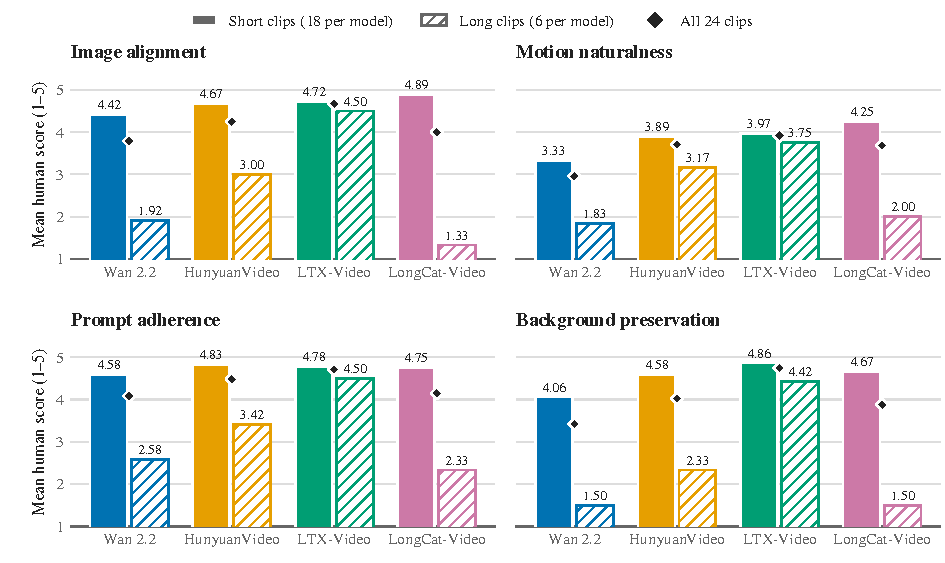
\includegraphics[width=\linewidth]{human_scores.pdf}
  \caption{Human scores split by clip length. Solid bars are short clips, hatched bars are long clips and diamonds mark the mean over all 24 clips. All models are close on short clips. On long clips LTX-Video loses at most 0.44 points, whereas Wan~2.2 and LongCat-Video fall below 2.0 on image alignment and background preservation.}
  \label{fig:human}
\end{figure}

\subsection{Short versus Long Clips}
The overall means hide the most important pattern in the data, which Figure~\ref{fig:human} makes visible. On the 18 short clips the models are close: image alignment ranges from 4.42 to 4.89 and prompt adherence from 4.58 to 4.83, and LongCat-Video is in fact the best model on image alignment (4.89) and motion naturalness (4.25). On the 6 long clips the models diverge. LTX-Video drops by 0.22 to 0.44 points depending on the criterion. HunyuanVideo~1.5 drops by 0.7 to 2.3 points. Wan~2.2 and LongCat-Video collapse: their image alignment falls to 1.92 and 1.33, and their background preservation to 1.50 each.

LTX-Video's overall lead in Table~\ref{tab:human} therefore comes almost entirely from the long clips, and LongCat-Video's middling overall rank combines the best short-clip scores with the worst long-clip scores. This comparison is descriptive. Only six cases are long, they differ in content from the short cases, and LongCat-Video's long clips also last 60\% longer in physical time, so the gap should not be read as a clean causal effect of length.

\subsection{Qualitative Comparison}
Figure~\ref{fig:qual-long} shows a long clip. All four models start from the same frame, and the differences appear within the first third of the clip. In the Wan~2.2 output the vegetation dissolves into a smooth blur and the runner shrinks and loses facial detail. LongCat-Video keeps a sharp subject but replaces him with a different person, without the lettering on the shirt, in front of a synthetic-looking textured background. HunyuanVideo~1.5 preserves the runner better but shows a regular moir\'e-like pattern in the vegetation. LTX-Video keeps the background texture close to the reference throughout. Its failure is of a different kind: the runner approaches the camera and has left the frame by the end of the clip. These observations match the human scores, in which raters penalised Wan~2.2 and LongCat-Video mostly on image alignment and background preservation.

\begin{figure}[!tb]
  \centering
  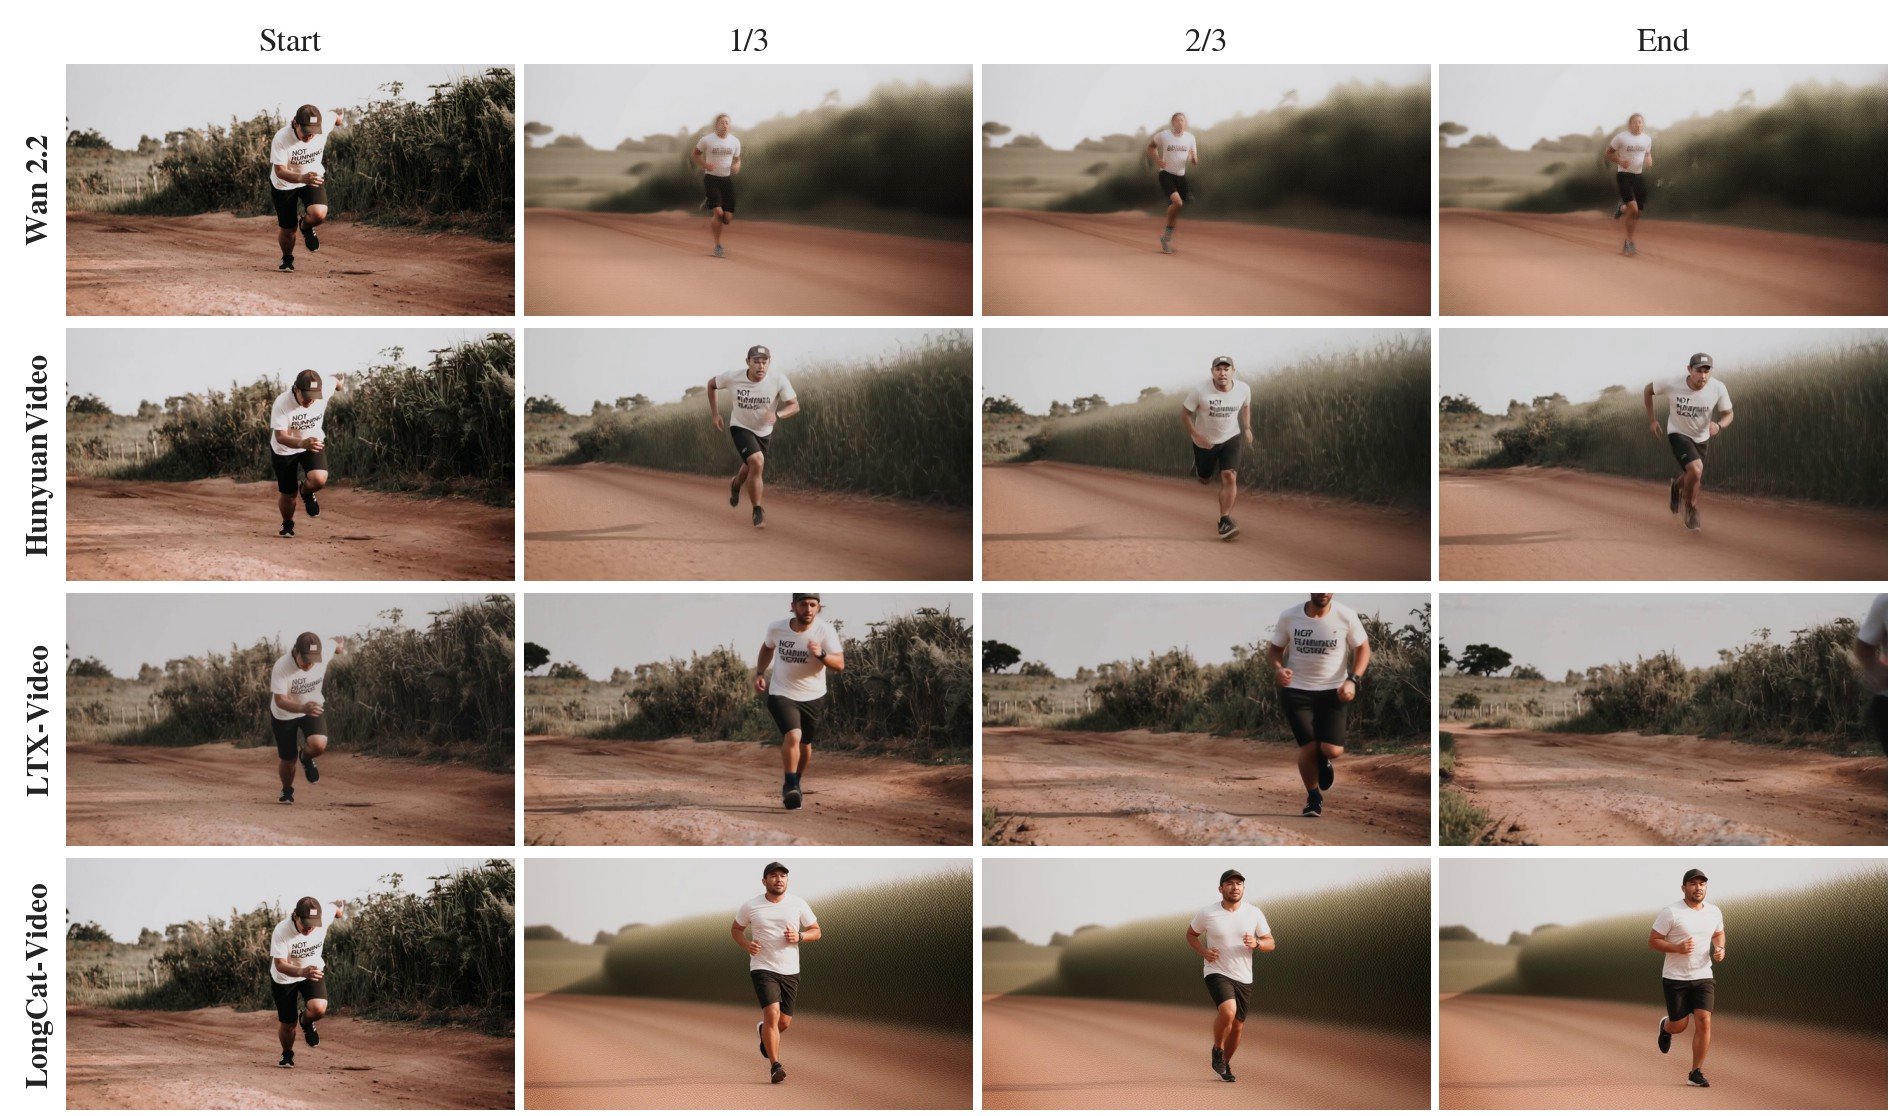
\includegraphics[width=\linewidth]{qualitative_long_running.jpg}
  \caption{Long clip, case 01, ``a man is running on a dirt road''. Frames are taken at the start, one third, two thirds and end of each clip. The first frame matches the reference image for all models.}
  \label{fig:qual-long}
\end{figure}

On short clips the differences are subtler (Figure~\ref{fig:qual-short}). All four models preserve the layout and the paintings of the gallery. They differ in how they introduce motion into a scene whose prompt requests none. HunyuanVideo~1.5 moves the camera and reveals a new wall, LTX-Video pans slowly, Wan~2.2 keeps the camera fixed and adds visitors who gather near the wall, and LongCat-Video changes little. Appendix~\ref{app:extra} shows the other five long clips and three further short clips.

\begin{figure}[!tb]
  \centering
  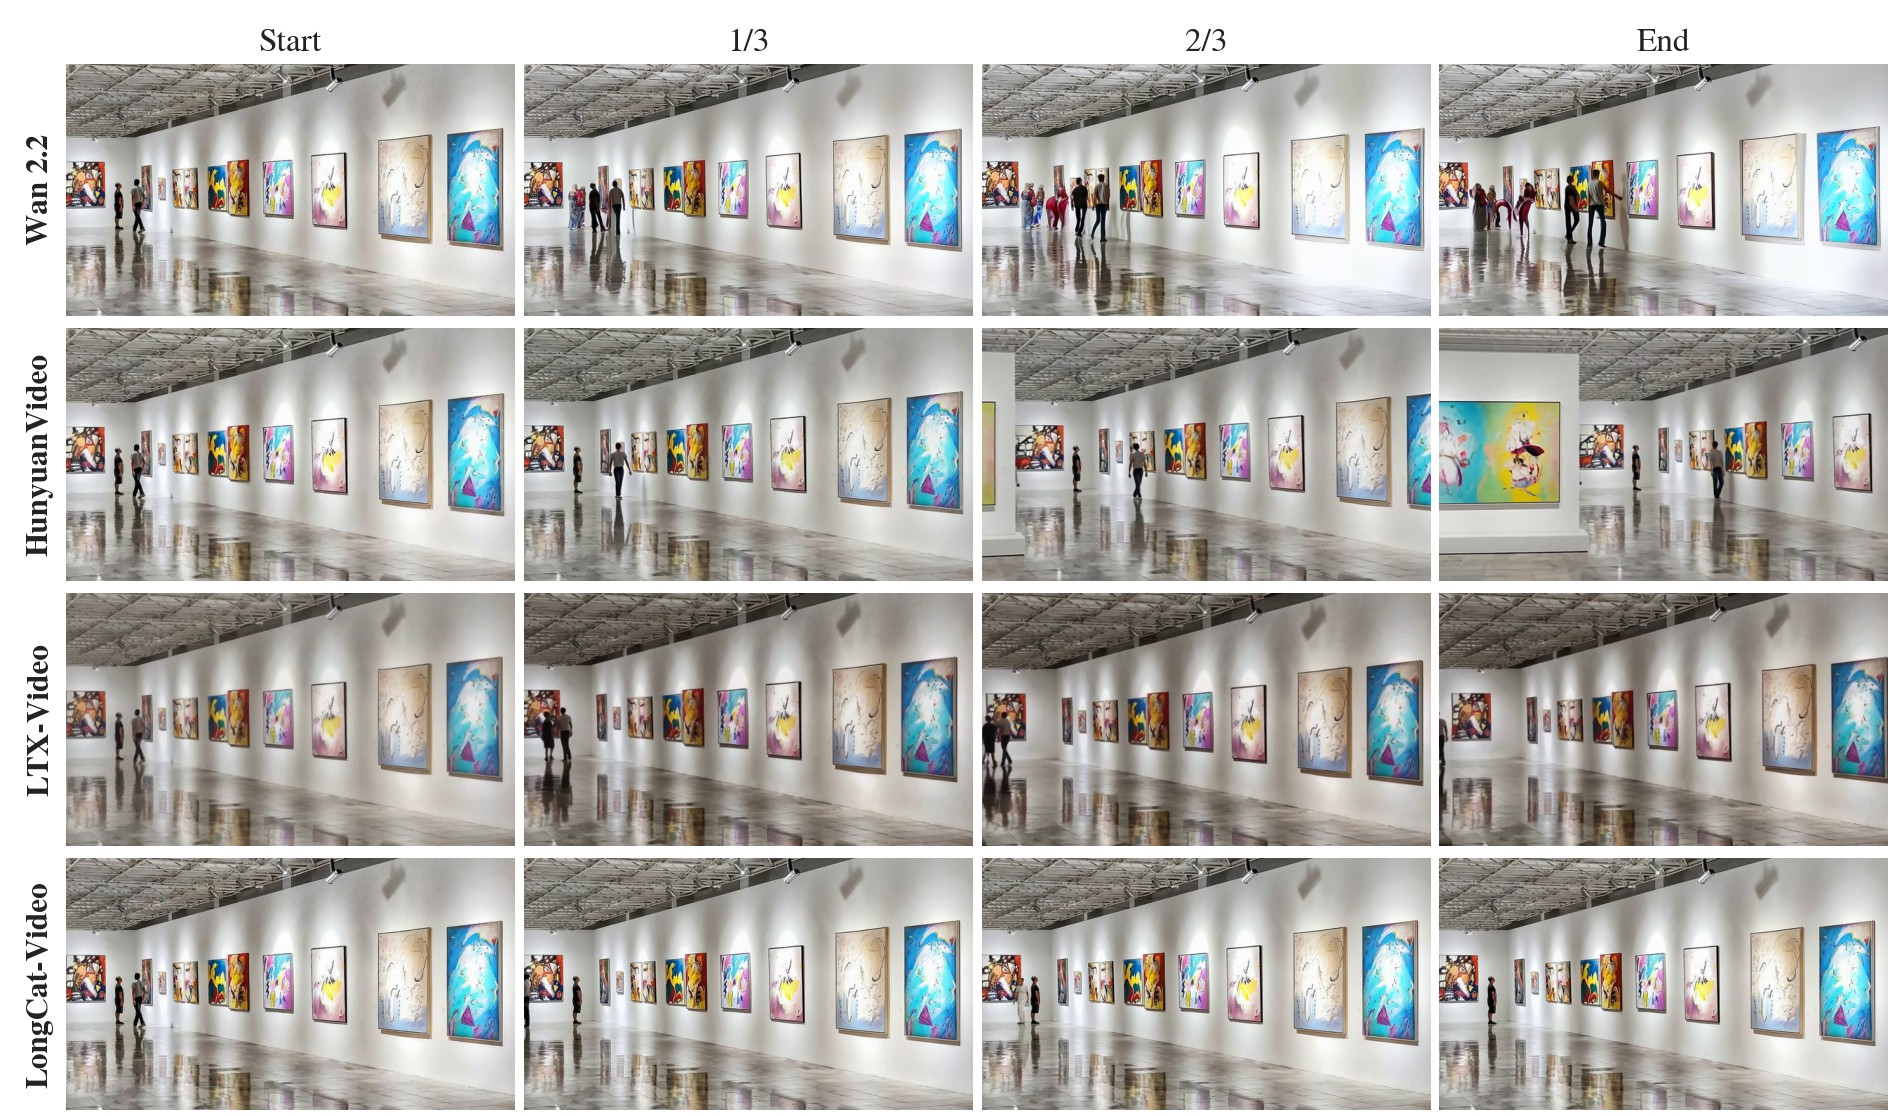
\includegraphics[width=\linewidth]{qualitative_short_gallery.jpg}
  \caption{Short clip, case 22, ``an art gallery with paintings on the walls''. All models preserve the scene, and they differ mainly in camera motion and in the people they add.}
  \label{fig:qual-short}
\end{figure}

\subsection{VBench-I2V Metrics}

\begin{table}[!htb]
  \centering
  \small
  \caption{VBench-I2V results (mean over applicable cases; higher is better for the first three columns). Dynamic degree measures the amount of motion and is not a quality score.}
  \label{tab:vbench}
  \begin{tabularx}{\linewidth}{@{}l Y Y Y Y@{}}
    \toprule
    & I2V subject ($n{=}16$) & I2V background ($n{=}8$) & Motion smoothness ($n{=}16$) & Dynamic degree ($n{=}16$) \\
    \midrule
    Wan~2.2          & \best{0.9787}   & \second{0.9760} & 0.9857          & 43.8\% \\
    HunyuanVideo~1.5 & \second{0.9730} & 0.9747          & \second{0.9904} & 68.8\% \\
    LTX-Video        & 0.9612          & \best{0.9811}   & \best{0.9917}   & 43.8\% \\
    LongCat-Video    & 0.9654          & 0.9637          & 0.9839          & 75.0\% \\
    \bottomrule
  \end{tabularx}
\end{table}

Table~\ref{tab:vbench} reports the automatic metrics. They compress the models into a narrow band, with all similarity and smoothness scores between 0.96 and 0.99, and they do not reproduce the human ranking. Wan~2.2 has the highest subject score although human raters place it last on image alignment. The metrics do agree with the raters that LTX-Video has the best background consistency and the smoothest motion, and they show that HunyuanVideo~1.5 and LongCat-Video move more (dynamic degree of 69\% and 75\%) than Wan~2.2 and LTX-Video (44\% each).

The disagreement follows from what the metrics measure. The subject and background scores reward global feature similarity to the reference image and between adjacent frames. A background that turns into a smooth blur changes slowly from frame to frame and stays globally similar to the reference, so it is penalised only mildly, and a person who is gradually replaced by another person of similar build and clothing is still the same subject in feature space. Across models, the Spearman correlation between a VBench metric and the corresponding human median is 0.50 for subject and image alignment ($n=64$), 0.37 for smoothness and motion naturalness ($n=64$), and 0.24 for the two background measures ($n=32$). Dynamic degree is uncorrelated with motion naturalness ($\rho=-0.07$): more motion is not better motion.

\subsection{Can a VLM Judge Replace Human Raters?}

\begin{table}[!htb]
  \centering
  \small
  \caption{Qwen3-VL scores (mean over 24 clips, scale 1--5) and their agreement with the human medians over all 96 videos. Bias is the mean of Qwen minus human.}
  \label{tab:qwen}
  \begin{tabularx}{\linewidth}{@{}l Y Y Y Y@{}}
    \toprule
    & Image alignment & Motion naturalness & Prompt adherence & Background preservation \\
    \midrule
    Wan~2.2          & 4.54        & \best{3.67} & 4.58        & 4.29 \\
    HunyuanVideo~1.5 & 4.75        & 3.33        & 4.88        & \best{4.88} \\
    LTX-Video        & \best{4.92} & 3.38        & \best{5.00} & 4.79 \\
    LongCat-Video    & 4.29        & 3.63        & 4.54        & 4.13 \\
    \midrule
    Spearman $\rho$ with human & 0.60 & $-0.06$ & 0.51 & 0.43 \\
    Mean absolute difference   & 0.46 & 1.84    & 0.43 & 0.67 \\
    Bias (Qwen $-$ human)      & $+0.45$ & $-0.07$ & $+0.40$ & $+0.51$ \\
    \bottomrule
  \end{tabularx}
\end{table}

\begin{figure}[!tb]
  \centering
  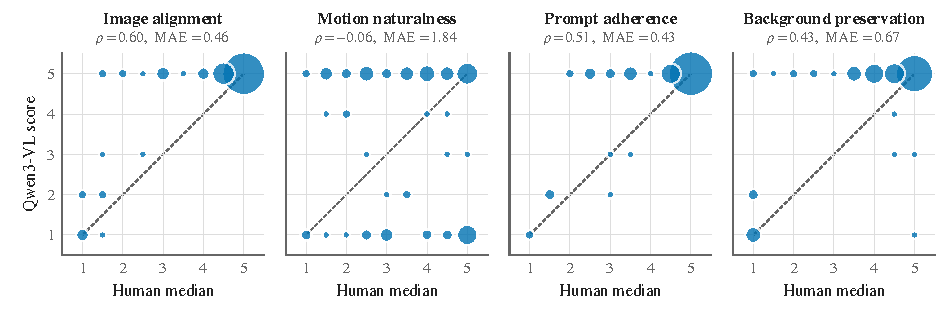
\includegraphics[width=\linewidth]{qwen_vs_human.pdf}
  \caption{Qwen3-VL score against the human median for each of the 96 videos. Marker area is proportional to the number of videos and the dashed line marks equality. The judge gives the top score to most videos. For motion naturalness its scores are spread over the whole scale independently of the human median.}
  \label{fig:qwen}
\end{figure}

Table~\ref{tab:qwen} and Figure~\ref{fig:qwen} compare the Qwen3-VL judge with the human medians. On image alignment, prompt adherence and background preservation the judge is lenient, scoring 0.4 to 0.5 points higher than the raters on average, but it is informative: its scores correlate with the human medians at $\rho=0.43$ to $0.60$, and it identifies LTX-Video as the best model on image alignment and prompt adherence. It also detects the long-clip collapse, giving LongCat-Video a mean image-alignment score of 2.17 on long clips against 5.00 on short ones.

Motion naturalness is different. The judge's motion scores have essentially no rank correlation with the human medians ($\rho=-0.06$) and differ from them by 1.84 points on average. The mean bias is close to zero, so the two sets of scores have similar averages while disagreeing on individual videos. An average that looks calibrated says nothing about per-video validity. With the judge's motion scores Wan~2.2 would rank first, whereas human raters rank it last.

Control experiments run during development point to the cause. An earlier 8-billion-parameter judge gave the top motion score to 65 of 72 videos. In a control experiment on six videos, it returned the top motion score in all 18 trials, whether it was shown the original video, a frozen first frame or a fully shuffled frame sequence. The 32B judge used for the final scores is better at recognising replaced subjects and degraded backgrounds but still failed to flag shuffled frame order and hand defects in our development checks. A model that reads sparsely sampled frames as a set of images can verify what is in the video, which is enough for alignment and prompt adherence, but it has little access to how things move. We therefore treat the judge's motion scores as a diagnostic of the method and do not use them to rank models.

\subsection{Computational Cost}

\begin{table}[!htb]
  \centering
  \small
  \caption{Mean generation time and peak allocated GPU memory per clip. Times for HunyuanVideo~1.5, LTX-Video and LongCat-Video are per-case wall-clock times of the generation worker. Wan~2.2 times cover sampling and decoding only, and its memory use was not logged.}
  \label{tab:cost}
  \begin{tabularx}{\linewidth}{@{}l c Y Y Y Y Y@{}}
    \toprule
    & & \multicolumn{2}{c}{Time per clip (s)} & Time per frame (s) & \multicolumn{2}{c}{Peak memory (GiB)} \\
    \cmidrule(lr){3-4}\cmidrule(lr){5-5}\cmidrule(l){6-7}
    Model & GPU & Short & Long & Short & Short & Long \\
    \midrule
    Wan~2.2          & A40  & 464        & 1{,}823      & 3.71        & 28.9          & 44.4 \\
    HunyuanVideo~1.5 & L40S & 173        & 1{,}145      & 1.34        & 32.7        & \best{33.2} \\
    LTX-Video        & L40S & \best{25}  & \best{206}   & \best{0.19} & \best{29.7} & 36.9 \\
    LongCat-Video    & L40S & 447        & 3{,}747      & 3.47        & 34.7        & 37.3 \\
    \bottomrule
  \end{tabularx}
\end{table}

Table~\ref{tab:cost} summarises the cost of generation. LTX-Video is faster than the other models by a wide margin. It needs 25\,s for a short clip, about 7 times less than HunyuanVideo~1.5 and 18 times less than Wan~2.2 and LongCat-Video, and it generates a 21-second clip in under four minutes. This is consistent with its highly compressed latent space and 10-step schedule. LongCat-Video is the slowest on long clips, at just over an hour each, partly because 40 of its 48 transformer blocks had to be offloaded to CPU memory to fit a 513-frame sequence on one GPU. All  models with memory logs peak between 30 and 45\,GiB, so each needs a 48\,GB card in these configurations.

The timings are not a controlled benchmark. Wan~2.2 ran on an A40 at a higher resolution and with classifier-free guidance, which doubles the number of network evaluations per step, and the models use different offloading strategies. The ordering is nevertheless large enough to be robust to these differences. In our setting quality and cost do not trade off: the cheapest model is also the one with the best human scores.

% =====================================================================
\section{Discussion and Limitations}
\label{sec:discussion}

\paragraph{What the comparison shows.}
Three observations hold across the evaluators. First, on clips of about five seconds the four models are of similar quality, and the choice between them can be made on cost. Second, extending the clip to about twenty seconds in a single pass exposes large differences in temporal stability that short-clip benchmarks do not reveal. Third, the typical long-clip failure is a gradual loss of the reference content: backgrounds lose texture and subjects are replaced. The model that avoided this failure in our tests, LTX-Video, did so at a fraction of the cost of the others.

\paragraph{What it does not show.}
The study has several limitations that restrict how far the results generalise.
\begin{itemize}
  \item \textbf{Sample size.} There are 24 cases, one seed and one video per case, and only six long clips per model. Category-level conclusions are not supported, and no significance tests were run.
  \item \textbf{Unequal settings.} Step counts (10, 8, 7+3 and 16), resolutions and frame rates differ, three checkpoints are distilled and one is not, and Wan~2.2 ran below its default budget. The results rank these configurations, not the model families.
  \item \textbf{Long clips are out of distribution.} A single 513-frame pass exceeds the clip lengths the models were designed for. LongCat-Video in particular is intended to reach long durations through video continuation, which we did not use.
  \item \textbf{Rater reliability and blinding.} Agreement is moderate ($\alpha$ of 0.54 to 0.66), and raters could sometimes recognise the videos they had generated. The owner-excluded analysis reduces this concern but does not remove it.
  \item \textbf{Evaluator inputs differ.} Human raters watched native-frame-rate copies, VBench used 12\,fps copies, and the VLM judge sampled frames from the native files, so the three evaluators did not see exactly the same pixels.
\end{itemize}

\paragraph{Implications for evaluation.}
The automatic evaluators were most useful for properties that can be checked on individual frames and least useful for motion. VBench's similarity metrics saturate near 1.0 and miss slow degradation, and the VLM judge cannot yet assess temporal order. Until VLM judges are validated on held-out videos with known defects, human rating remains necessary for motion quality, and reporting rater agreement alongside the means is needed to show how much weight the scores can bear.

% =====================================================================
\section{Conclusion}
We compared Wan~2.2, HunyuanVideo~1.5, LTX-Video and LongCat-Video on 24 shared VBench-I2V cases with human, metric-based and VLM-based evaluation. On short clips all four models preserve the reference image and follow the prompt well, with LongCat-Video slightly ahead on image alignment and motion. On long clips only LTX-Video remains stable, while Wan~2.2 and LongCat-Video lose most of the reference content. LTX-Video is also 7 to 18 times faster than the other models on short clips. VBench-I2V metrics and a Qwen3-VL judge capture image alignment and prompt adherence to a useful degree, but neither reflects human judgement of motion, and the judge's motion scores are uncorrelated with it. Future work should repeat the comparison with multiple seeds, matched sampling budgets and each model's intended long-video mode, and should validate VLM judges on a held-out set of videos with annotated temporal defects.

% =====================================================================
{\small
\bibliographystyle{unsrtnat}
\bibliography{references}
}

% =====================================================================
\appendix

\section{Human Scoring Rubric}
\label{app:rubric}
Each criterion is scored independently on a five-point scale. Table~\ref{tab:rubric} gives the two anchors, and scores of 2, 3 and 4 indicate intermediate levels. Raters were instructed to check hands, feet, contact and sliding when judging motion, not to penalise brief and plausible motion blur, and to compare the background in the middle and late parts of the clip with the reference image, without letting a sharp subject compensate for a degraded background.

\begin{table}[!htb]
  \centering
  \small
  \caption{Anchors of the human scoring rubric, also given to the VLM judge.}
  \label{tab:rubric}
  \begin{tabularx}{\linewidth}{@{}>{\raggedright\arraybackslash}p{28mm} L L@{}}
    \toprule
    Criterion & 1 point & 5 points \\
    \midrule
    Image alignment &
      The subject or scene changes substantially. A person, if present, is replaced or is hard to recognise as the original subject. &
      Key attributes of the subject's appearance and of the scene remain stable throughout. Visible changes are consistent with the action or viewpoint. \\
    \addlinespace
    Motion naturalness &
      Severe stutter, abrupt jumps or structural deformation, or an action explicitly requested in the prompt is largely absent. &
      Motion is continuous and coherent with discernible local detail. Speed, trajectories and physical contact are plausible for the scene. \\
    \addlinespace
    Prompt adherence &
      The main requirements are missing or clearly contradicted by the video. &
      The main requirements on subject, action and scene are all verifiable in the video. \\
    \addlinespace
    Background preservation &
      Nearly all initially identifiable background structure or texture is lost, the background stays severely blurred, or the scene changes without a clear reason. &
      Major background structures, edges and textures are largely preserved wherever they are visible and comparable with the reference image. \\
    \bottomrule
  \end{tabularx}
\end{table}

\section{Additional Qualitative Examples}
\label{app:extra}
This appendix shows the remaining five long clips, so that together with Figure~\ref{fig:qual-long} all six long cases are covered, followed by three further short clips. Each example is described first and shown directly below. All figures use the layout of Figure~\ref{fig:qual-long}, with frames taken at the start, one third, two thirds and end of each clip. The scores quoted are medians of the four human raters.

\subsection{Long Clips}

\qualexample{Two people}{fig:qual-boxing}{qualitative_long_boxing.jpg}
  {Long clip, case 04, ``a man and a woman are boxing in a boxing ring''.}
  {LongCat-Video and HunyuanVideo~1.5 replace one or both people, and Wan~2.2 loses facial and clothing detail. Their image-alignment scores are 1.0, 1.5 and 1.5. LTX-Video keeps both people recognisable (4.5) although the framing changes. Individual raters gave the HunyuanVideo~1.5 output 1, 3, 1 and 2 on this criterion, yet its VBench I2V-subject score is 0.971, which illustrates the gap between global feature similarity and the identity of the people in the scene.}

\qualexample{Animal}{fig:qual-giraffe}{qualitative_long_giraffe.jpg}
  {Long clip, case 07, ``a giraffe walking in a field''.}
  {The giraffe itself survives in all four outputs, and the differences lie in the background. Wan~2.2 and LongCat-Video reduce the savannah to a defocused blur (background preservation 1.0 for both). HunyuanVideo~1.5 keeps the animal sharp but flattens the vegetation (2.5). LTX-Video retains the grass and tree texture (4.5) while the scene drifts as the camera follows the animal.}

\qualexample{Vehicle in a complex scene}{fig:qual-train}{qualitative_long_train.jpg}
  {Long clip, case 09, ``a blue train traveling through a lush green area''.}
  {This is the hardest long case, and no model exceeds 3.0 on image alignment. LongCat-Video discards the scene and leaves a train on a featureless green surface (1.0). Wan~2.2 turns the hillside into a soft painterly texture (2.0). HunyuanVideo~1.5 shows a dissolve-like artefact around the station building in the middle of the clip (2.5). LTX-Video stays sharp, but the camera moves and the layout of the scene changes (3.0), so that prompt adherence remains high (4.5) while alignment with the reference image does not.}

\qualexample{Static scenery}{fig:qual-waterfall}{qualitative_long_waterfall.jpg}
  {Long clip, case 19, ``a large waterfall in the middle of a lush green hillside''.}
  {The long-clip collapse is not universal. On this nearly static scene Wan~2.2 and HunyuanVideo~1.5 hold the composition for the whole clip (image alignment 4.5 and 5.0), and LTX-Video scores 4.5 despite a slow camera rise that changes the framing. LongCat-Video is the exception: the cliffs lose their rock and grass structure and turn into smooth shapes (image alignment 1.5, background preservation 1.0).}

\qualexample{Abstract texture}{fig:qual-abstract}{qualitative_long_abstract.jpg}
  {Long clip, case 23, ``A black and white abstract video featuring mesmerizing bubbles''.}
  {This case gives the clearest separation. In the Wan~2.2, HunyuanVideo~1.5 and LongCat-Video outputs the pattern has vanished by one third of the clip and is replaced by a flat gradient, and all three receive 1.0 on image alignment and background preservation. LTX-Video keeps a moving bubble pattern with the original palette throughout (5.0 on both).}

\subsection{Short Clips}

\qualexample{Tool use}{fig:qual-salmon}{qualitative_short_salmon.jpg}
  {Short clip, case 12, ``a person slicing salmon on a cutting board''.}
  {Every model keeps the hands, knife and fish consistent with the reference image (image alignment 5.0 for all) and produces a slicing action. Motion naturalness ranges from 3.5 for Wan~2.2 to 5.0 for HunyuanVideo~1.5.}

\qualexample{Fine hand motion}{fig:qual-knitting}{qualitative_short_knitting.jpg}
  {Short clip, case 05, ``an older woman and a young girl are knitting together''.}
  {All four models keep both people and the room recognisable (image alignment 4.5 to 5.0). They differ in the knitting action itself. HunyuanVideo~1.5 and LongCat-Video receive 4.0 on motion naturalness, whereas Wan~2.2 and LTX-Video receive 2.5 and 2.0 because the hands and needles are blurred and their movement is hard to follow during playback, which still frames show only in part. Wan~2.2 also brightens and simplifies the area behind the subjects (background preservation 2.0). The Qwen3-VL judge gave the LTX-Video clip a motion score of 4, which makes it one of the cases where the judge and the raters disagree.}

\qualexample{Free-moving subject}{fig:qual-turtle}{qualitative_short_turtle.jpg}
  {Short clip, case 08, ``a sea turtle swimming in the ocean under the water''.}
  {The models choose different trajectories from the same starting frame. In the Wan~2.2 output the turtle swims away from the camera, in the HunyuanVideo~1.5 output it approaches, in the LTX-Video output it turns side-on, and LongCat-Video adds a reflection at the water surface. All four receive 5.0 on image alignment and 4.0 to 5.0 on motion naturalness, so on short clips the same input can lead to quite different motion that raters find equally acceptable.}

\end{document}
